\chapter{}


\section{Techno-Economy Assessment}
\label{sec:techno_eco}

\subsection{Budget}
The comparison between the proposed and actual budget is discussed and why the project was under-budget.\\

The proposed budget for the project was R19,700. This budget was planned to cover cost of purchasing sensors, components, software and the manufacturing of the mechanical and electronic hardware. Table \ref{table:budget} provides the categories and amounts of what the actual budget consisted out of.\\

\begin{table}[h]
	\centering
	\begin{tabular}{|c|c|c|}
		\hline
		Category & Actual Budget & Proposed Budget \\
		\hline
		\hline
		Electronic Components & R2,019 & R2,500\\
		\hline
		Mechanical Components & R600 & R4,000\\
		\hline 
		Software & R0 & R800\\
		\hline
		Mechanical Manufacturing & R8,000 & R10,000\\
		\hline
		Electronic Manufacturing & R1000 & R2,400\\
		\hline
		\hline 
		Total & R11,619 & R19,700\\
		\hline
		
	\end{tabular}
	\caption{Categories of the Budget }
	\label{table:budget}
	
\end{table}

It is visible in Table \ref{table:budget} that the project is under-budget. The reason for being under-budget is due the Electrical and Electronic (E\&E) Deparment providing the services and components which were most expensive. This includes the manufacturing of the mechanical parts and PCB. The Mechanical and Mechatronic Department provided the motor that was used in the project which significantly reduced the cost for acquiring the mechanical components.


\subsection{Planning}

\begin{figure}[h]
	\centering
	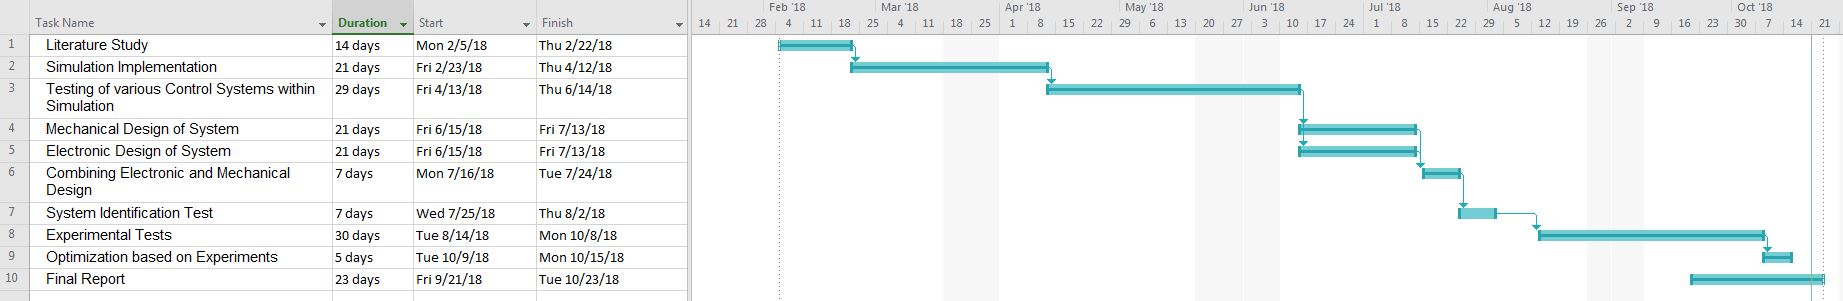
\includegraphics[scale=0.35]{./figs/planning_gantt/planned_ganttchart.jpg}
	\caption{Planned Gantt Chart of the Project}
	\label{fig:planned_ganttchart}
\end{figure}

\begin{figure}[h]
	\centering
	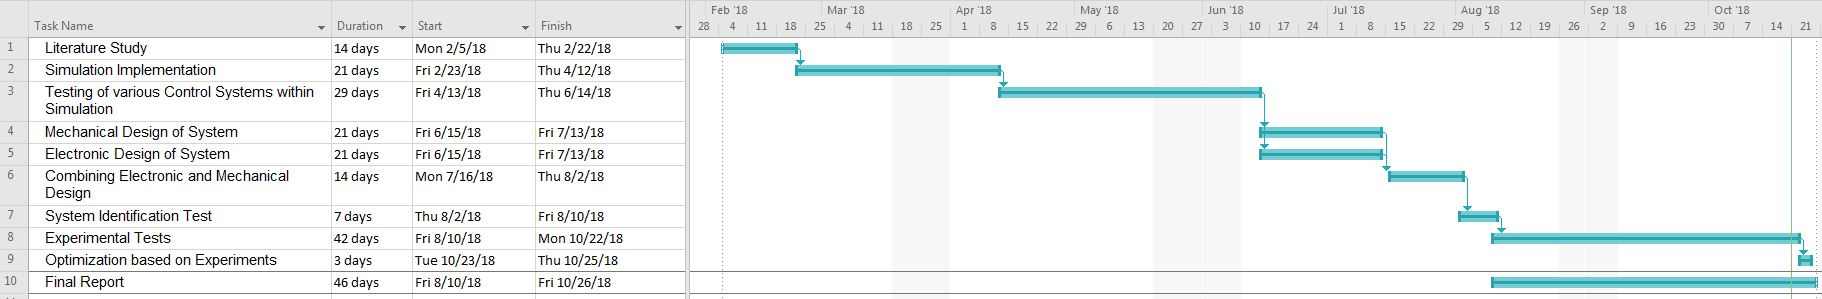
\includegraphics[scale=0.35]{./figs/planning_gantt/actual_ganttchart.jpg}
	\caption{Actual Gantt Chart of the Project}
	\label{fig:actual_ganttchart}
\end{figure}

\begin{table}[h]
	\centering
	\begin{tabular}{|c|c|c|}
		\hline
		Task Name & Planned Hours & Actual Hours \\
		\hline
		\hline
		Literature Study & 10 & 11 \\
		\hline
		Simulation Implementation & 15 & 12 \\
		\hline
		Testing \& Verification of Simulation & 20 & 20 \\
		\hline 
		Mechanical Design  & 50 & 51 \\
		\hline
		Electronic Design & 50 & 57 \\
		\hline
		Combining Electronic and Mechanical design & 84 & 83 \\
		\hline
		System Identification Test & 28 & 25 \\
		\hline
		Experiments & 192 & 192\\
		\hline
		Writing of Report & 112 & 192 \\
		\hline
		\hline
		Total & 561 & 643 \\
		\hline
		
	\end{tabular}
	\caption{Hours worked during the different phases of the project}
	\label{table:hours_worked}
\end{table}

Figure \ref{fig:planned_ganttchart} shows the Gantt chart for the planned activities during the project. For the majority of the project, the planned activities were followed as planned. These activities include the literature study up to the integrating the electronic and mechanical subsystems.\\

During the experimental testing it was required to improve the mounting method between the motor shaft and the actuated pendulum. During this modification the experiments could not continue and additional time was required. The decision to extend the time required for the experiments were justified by the increase of safety to the individual and surroundings during the experiments with the improved mounting method. It was also decided that during the improvement of the mounting method the writing of the report will start.\\	

The electronic design took longer than what was planned due to experiencing difficulty programming the theoretical controllers on the microcontroller. It was decided to extend the time required for this phase due to without the controllers no practical results of these controllers would be acquired. It was decided to take an additional week to implement the controllers.\\

\subsection{Technical Impact}
The impact of the results presented in this report on the field of control systems, society and industry are discussed and whether the financial input was worthwhile.\\

The swinging and balancing of the robotic gymnast is a well researched problem in control systems. Solutions to the swinging and balancing are provided on a theoretical level and supported by simulation results however little practical results are available of these theoretical solutions. The impact of this report on the field of control systems includes the possibility of future practical results of one of these theoretical solutions. It will enable the theoretical and practical results to be compared and the improvement of these controllers.\\

The impact of the practical results of this report on the industry of underactuated robotics are little. The robotic gymnast is a interesting research problem and consist out of a highly non-linear and linear behaviour and is rather consider a great introductory problem to the field of underactuated robotics. Method used for controlling underactuated robotics are more advance and build on the techniques describe in this report.\\

The impact of this report has little impact on society due to being of little interest to the industry. The industry will not use the results and discussion presented in this report due to the reasons mentioned in the previous paragraph.\\

The financial input was worthwhile due to the future possibility of practical results on theoretical implementation to the swinging and balancing of the robotic gymnast.\\


\subsection{Return on Investment}
The short and long term value from a technical and economical perspective is provided in this section. A motivation on the continuing research in the field of underactuated robotics are given and the financial cost to further research in this field.\\

Researching underactuated robotics is a exciting and growing research field due to the field of underactuated robotics have increasingly become more important due to technology growing in areas where control is crucial. Areas include: air drones, underwater inspection vehicles, space exploration and the aeroplane industry. \\

Underactuated robotics is an interesting and open field in control, with many design options to approach these types of problems. The most interesting examples of underactuated control problems are legged, swimming and flying robots that has been mentioned in the previous paragraph. This results in underactuated robotics being relevant in many fields.\\

The economical value of underactuated robotics in the short term and long term is high. Products are being brought to market that solve very difficult problems and can be used in a broad variety. These products include \textit{Spot} from \textit{Boston Dynamics} which can be used for inspection, transportation and entertainment. The market is open for more competitors to enter and results in long term value.\\

The financial cost to further the research on underactuated robotics are low due to the use of simulation programs that allows the testing of solutions on realistic simulated models. This significantly reduce the number of prototypes required to test the solution practically. 

\subsection{Potential for Commercialisation}\
The potential for the commercialisation of the contents within the report is discussed and the value of this commercialisations is given.\\

The contents does not have any real value for commercialisation. As mentioned earlier the problem researched is a very good introductory to underactuated robotics due to containing techniques that is a foundation for more advanced problems. 

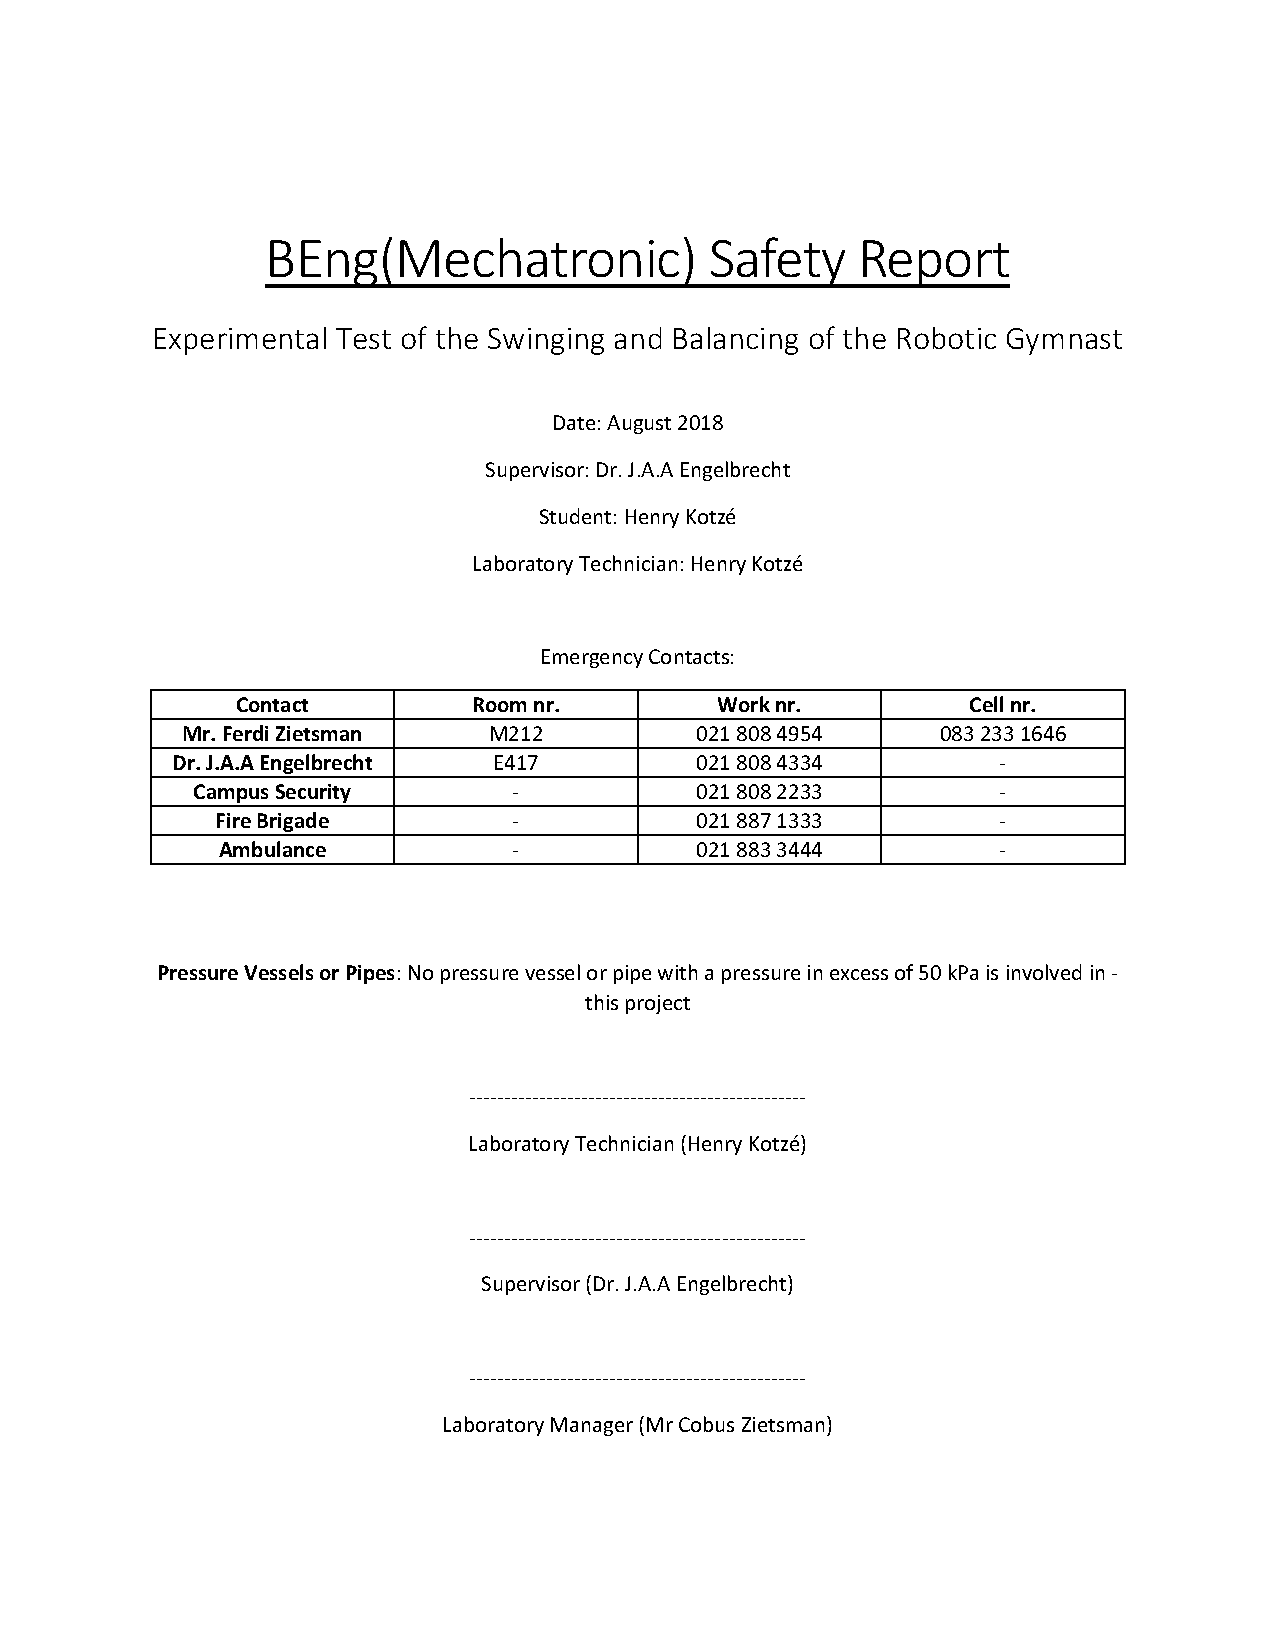
\includepdf[pages=1,pagecommand={\section{Risk Analysis \& Safety Procedures} \thispagestyle{empty} \label{sec:mech_drawings}}, fitpaper=true]{./figs/safety_report/safety_report.pdf}
\includepdf[pages=2-,pagecommand={\thispagestyle{empty}}, fitpaper=true]{./figs/safety_report/safety_report.pdf}
\begin{comment}
An outcome assessment must accompany the Final Report and included and bound into the
report after the summary page. This assessment is a single page on which the student must
indicate which parts of the report presents evidence of achieving each of the ECSA outcomes
(as specified in this document). A sentence or two can also be given for each outcome to
explain how those parts of the report demonstrate achieving the outcome
\end{comment}

\section{Derivation of the Mathematical Model}
\label{sec:math_model}

From the free body diagram shown in Figure \ref{fig:doublePen} the position of the center of mass of the unactuaded and actuaded pendulum can be determine as seen in equation (\ref{eq:pendulum_posx1}), (\ref{eq:pendulum_posy1}) , (\ref{eq:pendulum_posx2}) and (\ref{eq:pendulum_posy2}) respectively.

\begin{equation}
\label{eq:pendulum_posx1}
x_{1}= l_{1}\cos(\theta)
\end{equation}

\begin{equation}
\label{eq:pendulum_posy1}
y_{1} = -l_{1}\sin(\theta)
\end{equation}

\begin{equation}
\label{eq:pendulum_posx2}
x_{2} = L_{1}\sin(\theta) + l_{2}\sin(\theta + \phi)
\end{equation}

\begin{equation}
\label{eq:pendulum_posy2}
y_{2} = -L_{1}\cos(\theta) - l_{2}\cos(\theta + \phi)
\end{equation}

The Lagrange is defined as 
$$\mathcal{L}=T-V$$
where $T$ is the potential energy in the system and $V$ the kinetic energy.\\

The kinetic energy in the system consist of the fixed rotation of the unactuated  pendulum and the rotation and velocity of the actuated pendulum.

\begin{equation}
\label{eq:T}
T = \frac{1}{2}I_{A}\dot{\theta}^2 + \frac{1}{2}I_{B}(\dot{\theta}+\dot{\phi})^2 + \frac{1}{2}m_{2}V_{2}^2
\end{equation}

The potential energy in the system is defined as
$$V=-m_{1}gl_{1}\cos(\theta)-m_{2}g[L_{1}\cos(\theta)+l_{2}\cos(\theta+\phi)]$$

The velocity term $V_{2}$ in equation (\ref{eq:T}) must be expanded and this is accomplished by taken the derivative of equations (\ref{eq:pendulum_posx2}) and (\ref{eq:pendulum_posy2}).

$$\dot{x_{2}} = L_{1}\cos(\theta)\dot{\theta} - l_{2}\cos(\theta+\phi)(\dot{\theta}+\dot{\phi}) $$
$$\dot{y_{2}} = L_{1}\sin(\theta)\dot{\theta}+l_{2}\sin(\theta+\phi)(\dot{\theta}+\dot{\phi})$$

The $V_{2}$ term is the magnitude of the velocity of the actuated pendulum and results in the following expansion:

$$x_{2}^2 = L_{1}^2\cos(\theta)^2\theta^2 +l_{2}^2\cos(\theta+\phi)^2(\dot{\theta}+\dot{\phi})^2 + 2L_{1}l_{2}\dot{\theta}(\dot{\theta}+\dot{\theta})\cos(\theta)\cos(\theta+\phi)$$
$$y_{2}^2 = L_{1}^2\sin(\theta)^2\theta^2 +l_{2}^2\sin(\theta+\phi)^2(\dot{\theta}+\dot{\phi})^2 + 2L_{1}l_{2}\dot{\theta}(\dot{\theta}+\dot{\theta})\sin(\theta)\sin(\theta+\phi)$$

\begin{equation}
\label{eq:V_squared}
\begin{split}
V_{2}^2 = x_{2}^2+y_{2}^2 & = \\ &L_{1}^2\theta^2[\cos(\theta)^2+\sin(\theta)^2]+l_{2}^2(\dot{\theta}+\dot{\phi})^2[\cos(\theta+\phi)^2+\sin(\theta+\phi)^2] + \\
&2L_{1}l_{2}\dot{\theta}(\dot{\theta}+\dot{\phi})[\cos(\theta)\cos(\theta+\phi)+\sin(\theta)\sin(\theta+\phi)]
\end{split}
\end{equation}

Using the following trigonometric identities $$ \cos(\gamma)^2 + \sin(\gamma)^2 = 1 $$ 
$$ \cos(\gamma)\cos(\alpha)+\sin(\gamma)\sin(\alpha) = \cos(\gamma - \alpha) $$ the equation (\ref{eq:V_squared}) resolves to: $$ V_{2}^2 = L_{1}\dot{\theta}^2+l_{2}^2(\dot{\theta}+\dot{\phi})^2 + 
2L_{1}l_{2}(\dot{\theta}+\dot{\phi})\dot{\theta}\cos(\phi)$$

The kinectic energy in the system is then defined as:
$$ T = \frac{1}{2}I_{A}\dot{\theta}^2 + \frac{1}{2}I_{B}(\dot{\theta}+\dot{\phi})^2 + \frac{1}{2}m_{2}[L_{1}\dot{\theta}^2+l_{2}^2(\dot{\theta}+\dot{\phi})^2 + 
2L_{1}l_{2}(\dot{\theta}+\dot{\phi})\dot{\theta}\cos(\phi)]^2$$


and results in the Lagrangian to be:
$$\mathcal{L} = \frac{1}{2}I_{A}\dot{\theta}^2 + \frac{1}{2}I_{B}(\dot{\theta}+\dot{\phi})^2 + \frac{1}{2}m_{2}[L_{1}\dot{\theta}^2+l_{2}^2(\dot{\theta}+\dot{\phi})^2 + 
2L_{1}l_{2}(\dot{\theta}+\dot{\phi})\dot{\theta}\cos(\phi)]^2+m_{1}gl_{1}\cos(\theta)+$$
$$m_{2}g[L_{1}\cos(\theta)+l_{2}\cos(\theta+\phi)]$$

The differential equation describing the dynamics of the system is
$$\frac{d}{dt}\frac{\partial\mathcal{L}}{\partial\vec{\dot{q}}}-\frac{\partial\mathcal{L}}{\partial q} = B(\dot{q})+\tau(q)$$ 
where  $ q = 
\begin{bmatrix}
\theta \\
\phi
\end{bmatrix}
$

The appropriate derivatives are done and results in the equations 

\begin{equation}
\frac{\partial\mathcal{L}}{\partial\theta} = -m_{1}gl_{1}\sin(\theta)-m_{2}gL_{2}\sin(\theta)-m_{2}gl_{2}\sin(\theta+\phi)
\end{equation}

\begin{equation}
\begin{split}
\frac{d}{dt}\frac{\partial\mathcal{L}}{\partial\dot{\theta}} &=\\ &I_{A}\ddot{\theta}+I_{B}\ddot{\theta}+I_{B}\ddot{\phi}+m_{2}L_{1}^2\ddot{\theta}+m_{2}l_{2}^2\ddot{\theta}+\\
&m_{2}l_{2}\ddot{\phi}+2m_{2}L_{1}l{2}\ddot{\theta}\cos(\phi)-\\
&2m_{2}L_{1}l_{2}\dot{\theta}\dot{\phi}\sin(\phi)+\\
&m_{2}L_{1}l_{2}\ddot{\phi}\cos(\phi)-m_{2}L_{1}l_{2}\dot{\phi}^2\sin(\phi)
\end{split}
\end{equation}


\begin{equation}
\frac{\partial\mathcal{L}}{\partial\phi} = -m_{2}L_{1}l_{2}(\dot{\theta}+\dot{\phi})\dot{\theta}\sin(\phi)-m_{2}gl_{2}\sin(\theta+\phi)
\end{equation}

\begin{equation}
\begin{split}
\frac{d}{dt}\frac{\partial\mathcal{L}}{\partial\dot{\phi}} &= \\
&I_{B}\ddot{\theta}+I_{B}\ddot{\phi}+m_{2}l_{2}^2\ddot{\theta}+m_{2}l_{2}^2\ddot{\phi}+m_{2}L_{1}l_{2}\ddot{\theta}\cos(\phi)-m_{2}L_{1}l_{2}\dot{\theta}\dot{\phi}\sin(\phi)
\end{split}
\end{equation}

\begin{equation}
\frac{\partial\mathcal{L}}{\partial\phi} = -m_{2}L_{1}l_{2}(\dot{\theta}+\dot{\phi})\dot{\theta}\sin(\phi)-m_{2}gl_{2}\sin(\theta+\phi)
\end{equation}


\begin{equation}
\frac{d}{dt}\frac{\partial\mathcal{L}}{\partial\dot{\phi}}=I_{B}\ddot{\theta}+I_{B}\ddot{\phi}+m_{2}l_{2}^2\ddot{\theta}+m_{2}l_{2}^2\ddot{\phi}+m_{2}L_{1}l_{2}\ddot{\theta}\cos(\phi)-m_{2}L_{1}l_{2}\dot{\theta}\dot{\phi}\sin(\phi)
\end{equation}


\begin{comment}
\section{Collocated Linearisation}
\begin{equation} \label{app:eq:condense1}
d_{11}\ddot{\theta}+d_{12}\ddot{\phi} + h_{1} + \psi_{1} = 0
\end{equation}
\begin{equation} \label{app:eq:condense2}
d_{21}\ddot{\theta} + d_{22}\ddot{\phi} + h_{2} + \psi_{2} = \tau
\end{equation}

Starting from the condense equation (\ref{app:eq:condense1}) and (\ref{app:eq:condense2}), $\ddot{q_{1}}$ is solved in equation (\ref{app:eq:condense1}) and substituted in (\ref{app:eq:condense1}) resulting in 

\begin{equation} \label{app:eq:condense2}
\bar{d_{2}}\ddot{\theta} + \bar{h_{2}} + \bar{\psi_{2}} = \tau
\end{equation}
where the newly defined terms are given as: 
$$\bar{d_{2}} = d_{22} - \frac{d_{21}d_{12}}{d_{11}}$$
$$\bar{h_{2}} = h_{2} - \frac{d_{21}h_{1}}{d_{11}} $$
$$\bar{\psi_{2}} = \psi_{2} - \frac{d_{21}\psi_{1}}{d_{11}} $$


$\tau$ can now chosen to linearise the terms in equation (\ref{app:eq:condense2}) as:

$\tau = \bar{d_{2}}v_{2}+\bar{h_{2}} + \bar{\psi}$
\end{comment}

\section{Taylor Series Expansion Around Unstable Equilibrium Position}
\label{sec:linerisation}
The linearisation of equations (\ref{eq:condense1}) and (\ref{eq:condense2}) is by applying the Taylor Series Expansion at the working point:
\begin{equation}
	F(  \vec{q}, \dot{ \vec{q} }, \ddot{ \vec{q} } )  \approx  F(\vec{q_{s}},\dot{\vec{q_{s}}},\ddot{\vec{q_{s}}}) + \Delta( \vec{q}, \dot{ \vec{q} }, \ddot{ \vec{q} })\cdot \nabla F(\vec{q_{s}},\dot{\vec{q_{s}}},\ddot{\vec{q_{s}}})
\end{equation}
where the working point is defined as 
\begin{equation}
\label{eq:workingpoint}
[\vec{q_{s}},\dot{\vec{q_{s}}},\ddot{\vec{q_{s}}}]^{T}=[\pi,0,0,0,0,0]
\end{equation}
and 

\begin{equation}
\label{eq:workingpoint}
\Delta( \vec{q}, \dot{ \vec{q} }, \ddot{ \vec{q} }) =  [\vec{q}, \dot{ \vec{q} }, \ddot{ \vec{q} }] - [\vec{q_{s}},\dot{\vec{q_{s}}},\ddot{\vec{q_{s}}}]
\end{equation}

This results in the linearisation of equations (\ref{eq:condense1}) and (\ref{eq:condense2}) as :

\begin{equation}
\begin{split}
&(I_{A} + I_{B} + m_{2}L_{1}^2+m_{2}l_{2}+2m_{2}L_{1}l_{2})\Delta\ddot{\theta} + (I_{B}+m_{2}l_{2}^2+m_{2}L_{1}l_{2})\Delta\ddot{\phi}\\
&+(-m_{1}gl_{1}-m_{2}gL_{1}-m_{2}gl_{2})\Delta\theta -m_{2}gl_{2}\Delta\phi + f_{c1}\Delta\dot{\theta} = 0
\end{split}
\end{equation}

\begin{equation}
\begin{split}
&(I_{B}+m_{2}l_{2}^2+m_{2}L_{1}l_{2})\Delta\ddot{\theta} + (I_{B}+m_{2}l_{2}^2)\Delta\ddot{\phi}\\
& -m_{2}gl_{2}\Delta\theta -m_{2}gl_{2}\Delta\phi +f_{c2}(\Delta\dot{\phi}-\Delta\dot{\theta}) = \tau
\end{split}
\end{equation}

%\section{Additional Simulation Results}
%\label{app:simulation_results}











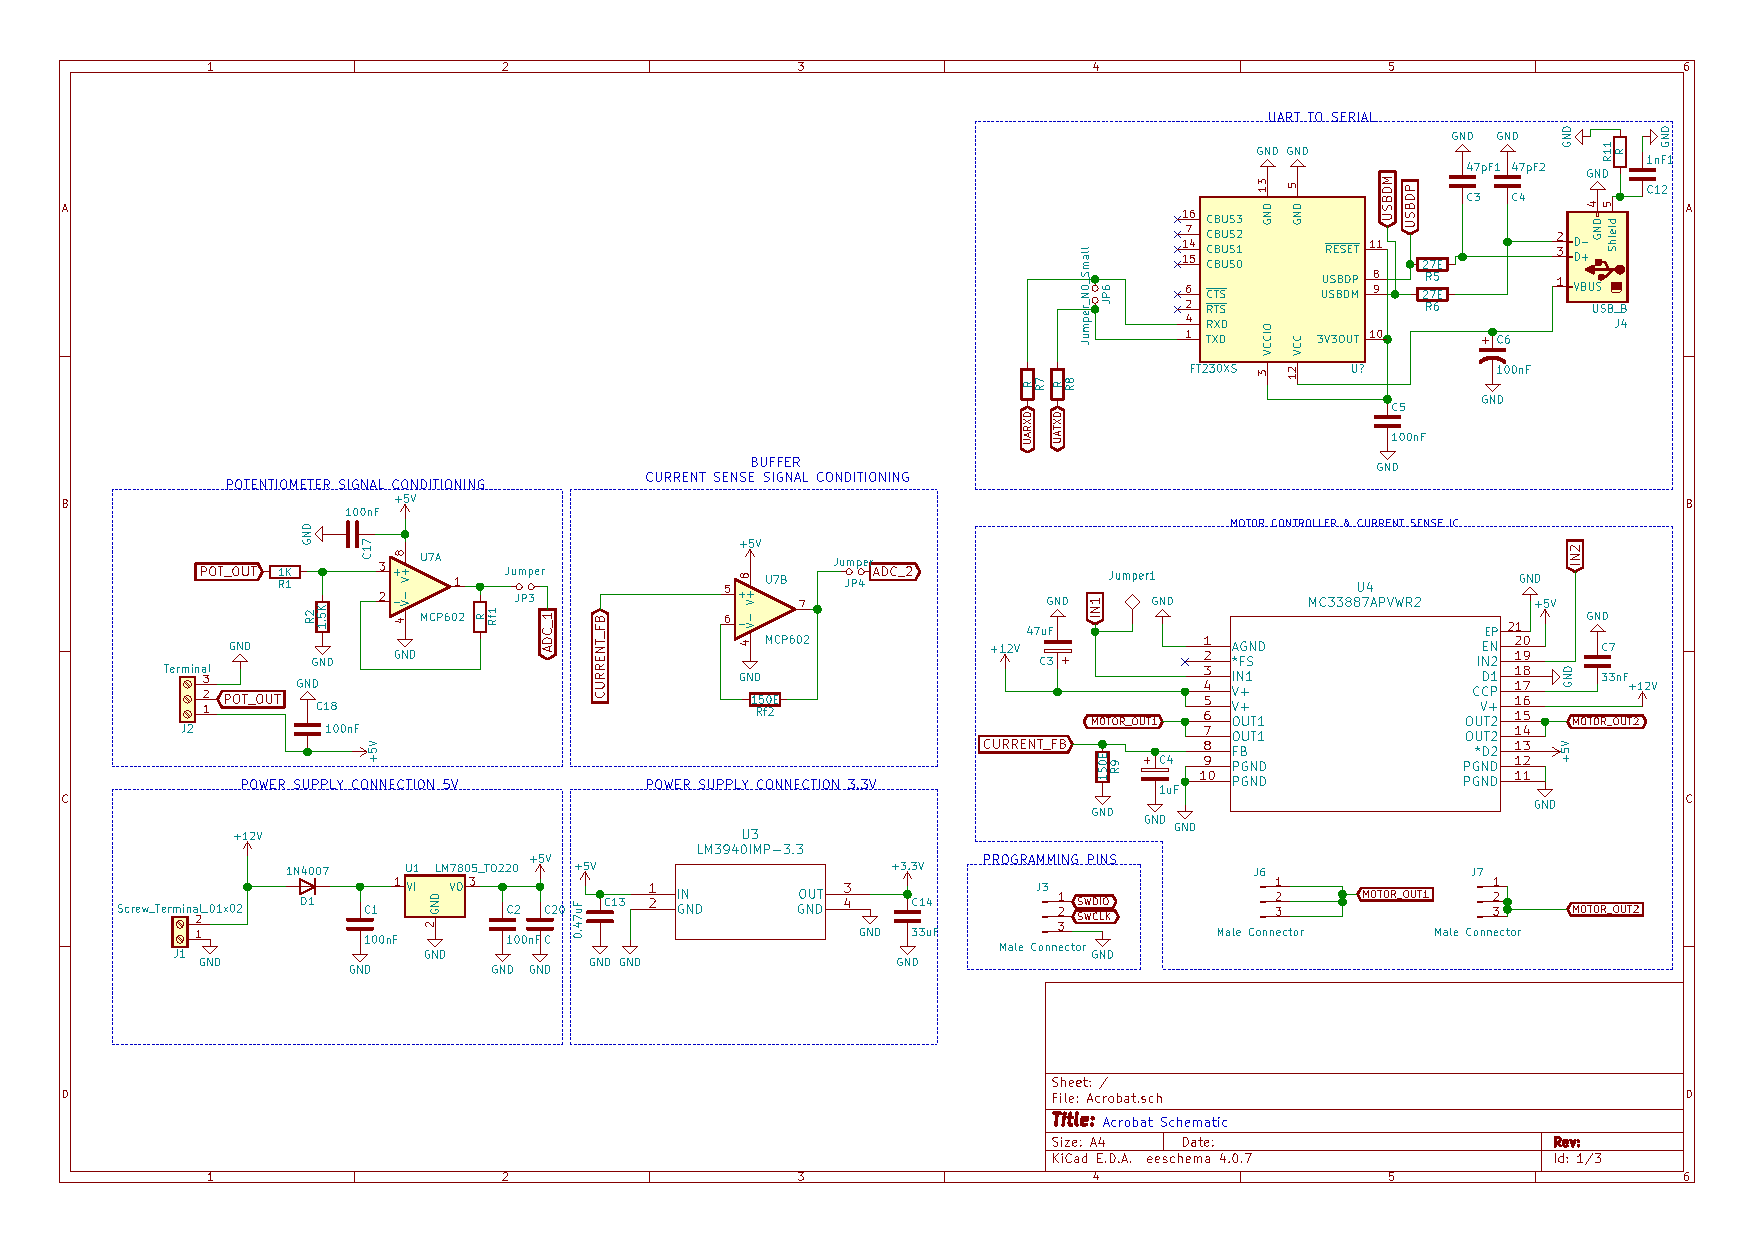
\includepdf[pages=1,pagecommand={\section{Electronic Design Schematic} \thispagestyle{empty} \label{sec:schematics}}, fitpaper=true]{./figs/Acrobat.pdf}
\includepdf[pages=2-,pagecommand={\thispagestyle{empty}}, fitpaper=true]{./figs/Acrobat.pdf}


\section{Communication Structure}
\label{sec:software_requirements}
\begin{figure}[h]
	\centering
	\begin{tikzpicture}[cell/.style={rectangle,draw=black},
	space/.style={minimum height=1.5em,matrix of nodes,row sep=-\pgflinewidth,column sep=-\pgflinewidth,column 1/.style={font=\ttfamily}},text depth=0.5ex,text height=2ex,nodes in empty cells]
	

	
	\matrix (first)[space, row 2/.style={minimum width=3em,nodes={cell,minimum width=3.5em}},row 3/.style={nodes={cell,minimum width=2em}}]
	{
		byte &0   & 1  & 2 & 3 & 4& \ldots & n-1&n  \\   
		&\$  & cmd  & , & value & value &  & \textbackslash r &  \textbackslash n \\};
	
	
	
	
\end{tikzpicture}
	\caption{Data Structure for Sending Commands}
	\label{fig:uart_struct_app}
\end{figure}

In Table \ref{table:uart_commands} the various commmands that are used in the command structure shown in Figure \ref{fig:uart_struct_app} used for debugging purposes is explained with the possible value ranges that can be used.


\begin{table}[h]
	\centering
	\begin{tabular}{|p{2cm}|p{1cm}|p{5cm}|p{5cm}|}
		\hline
		Command & Range &  Reason for Implementation & Effect \\
		\hline
		\hline
		A & None & Testing of the UART circuit & Send the following text: Feedback Control Of Robotic Gymnast\\
		\hline
		B & 0-1 & Used during experiments and system identification tests& Enable streaming of state variables across UART \\ 
		\hline
		F & 0-100 &  Testing AND digital circuit and speed control of motor& Changes PWM Duty-Cycle \\
		\hline
		I & 0-1 & Testing of AND digital circuit and directional control of motor & Change the rotational direction \\
		\hline
		X & None & Soft layer for safety & Stops all operation of microcontroller. A powercycle is required.   \\
		\hline
	
	\end{tabular}
	\caption{Summary of Communication Commands and their Effects}
	\label{table:uart_commands}

\end{table}


\newpage


%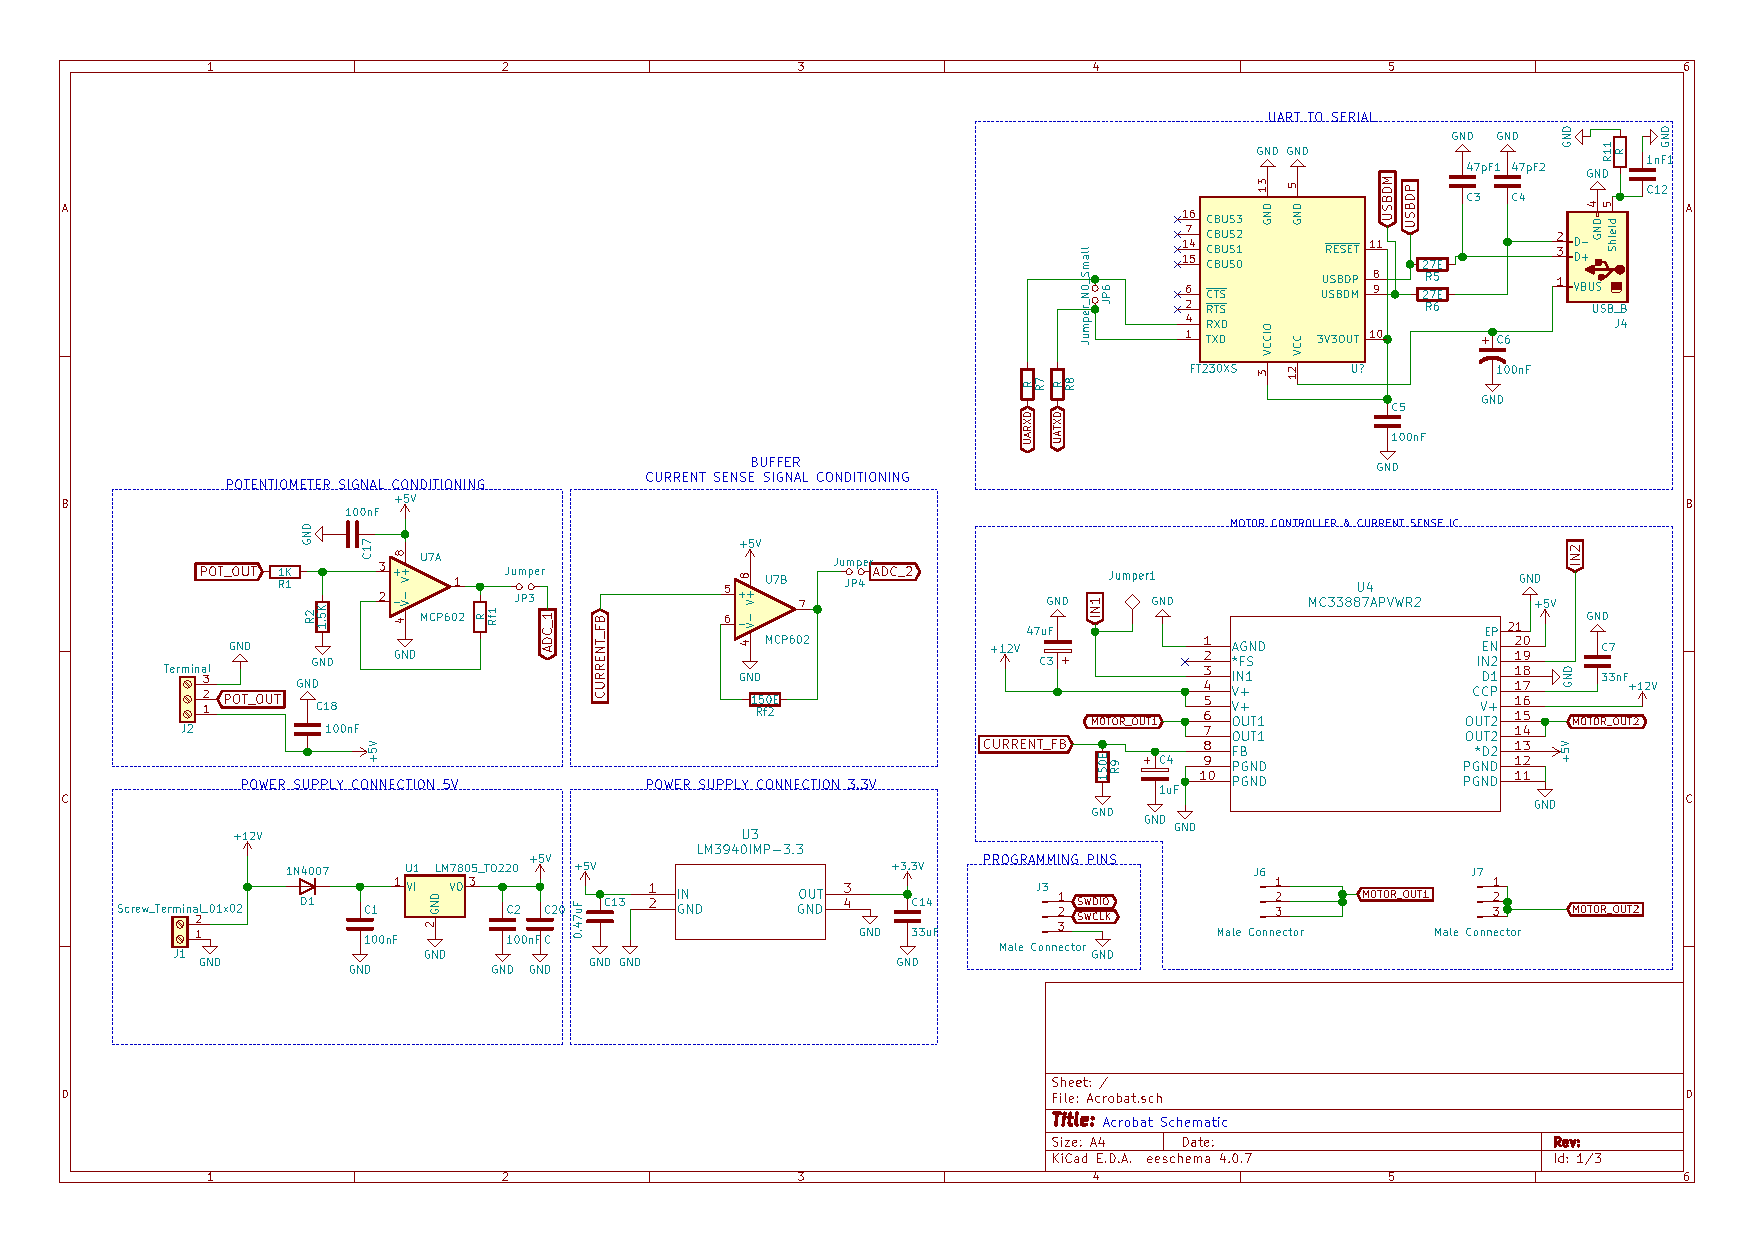
\includepdf[pages=-,scale-=0.8]{./figs/Acrobat.pdf}
%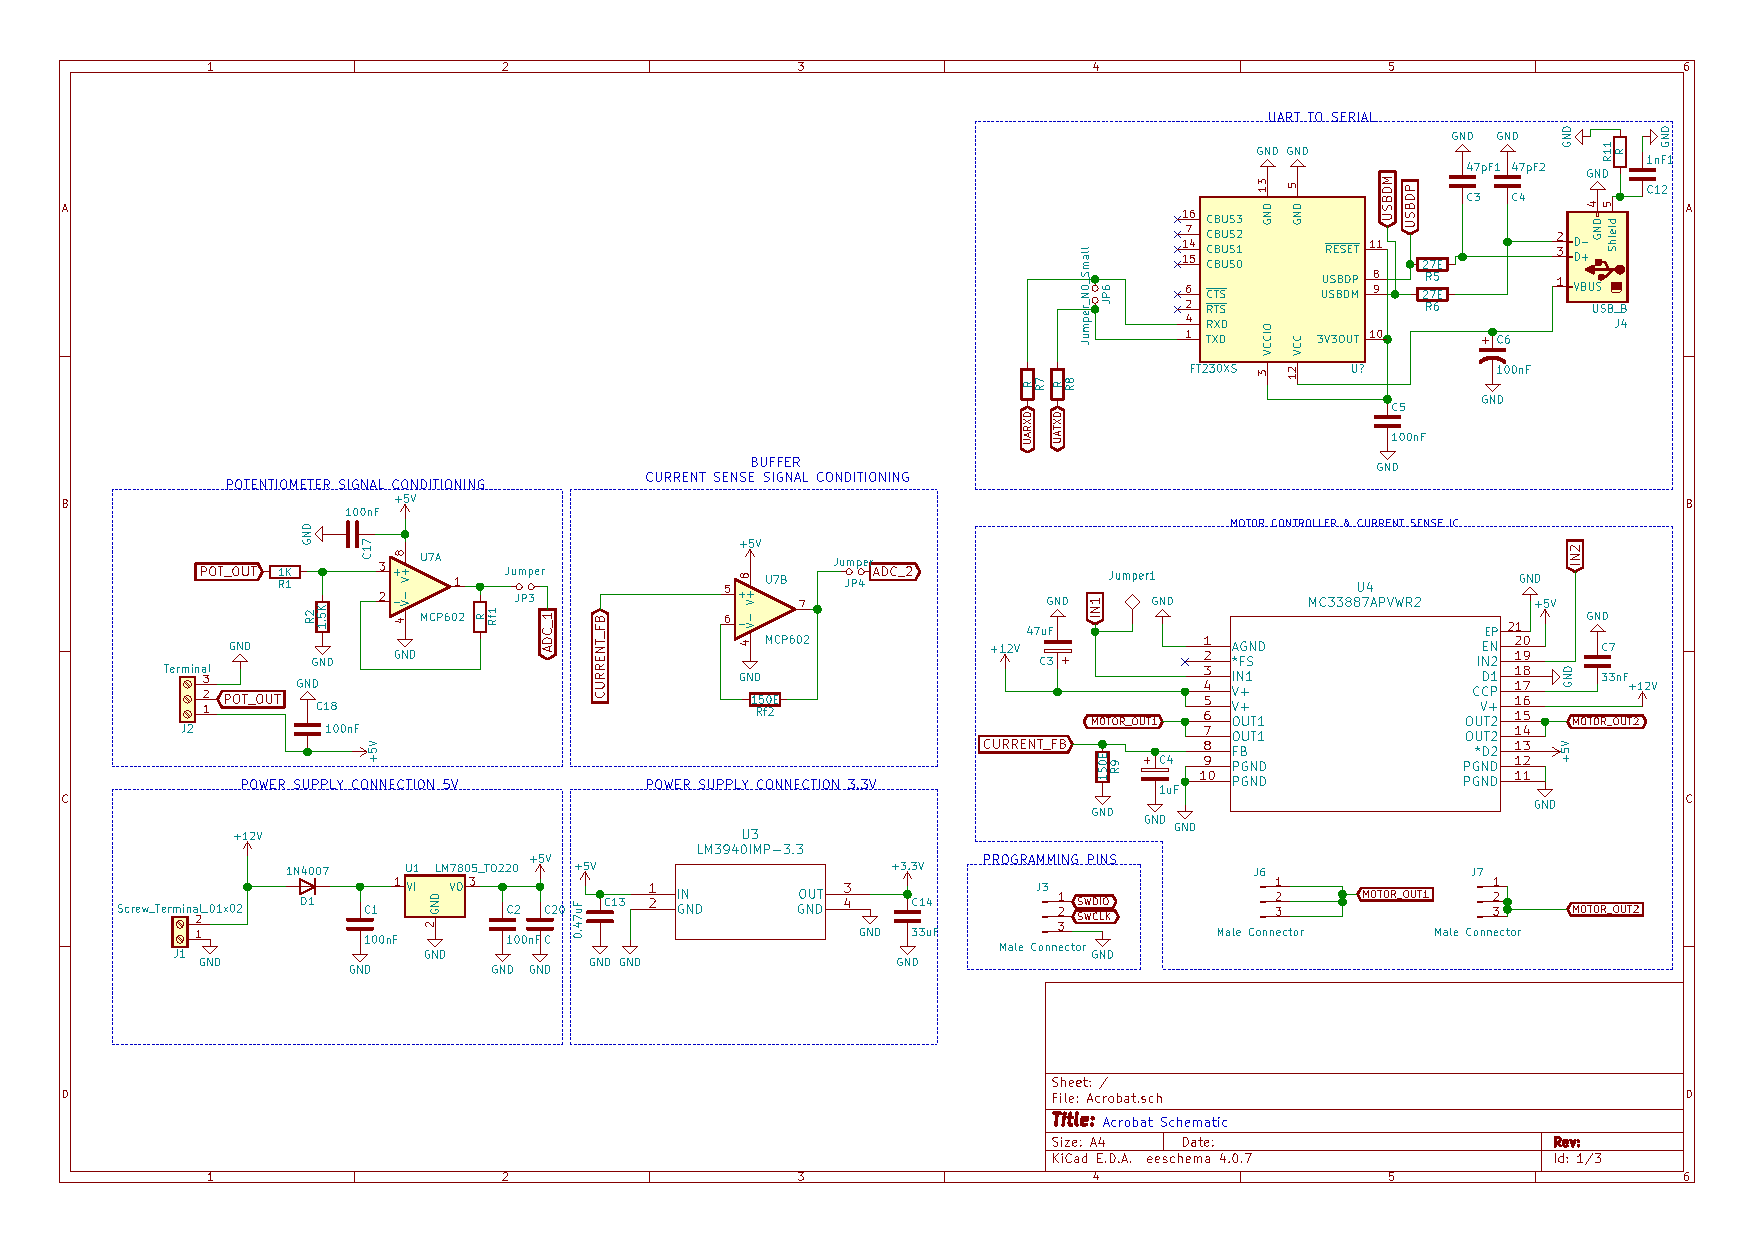
\includegraphics{./figs/Acrobat.pdf}







%----------------------------------------------------------------------------
\endinput
